\section{Exercise1}

This exercise investigates how the parameterization of a student neural
network relative to a teacher network affects its ability to learn.

\subsection{Setup}

We instantiate the teacher model $T$ as a fully connected neural network,
mapping a 100-dimensional input to a single output scalar, with three hidden
layers of 75, 50, 10 neurons respectively. 
We then instantiate three student models $S_1, S_2, S_3$ as fully connected neural
networks with the following architectures:
\begin{align*}
    S_1 &\text{ : 100-10-1}
    \\
    S_2 &\text{ : 100-75-50-10-1}
    \\
    S_3 &\text{ : 100-200-200-200-100-1}
\end{align*}
After doing so with proceed by generating
the testing data by sampling from the teacher model.
\begin{align*}
    D_{test} &= \{(x_i, T(x_i))\}_{i=1}^{N}
    \\
    x_i &\sim \mathcal{U}(0, 2)^{100}
    \\
    N &= 6 \cdot 10^4
\end{align*}
Conversely, the training data is generated lazily by sampling from the teacher
during training. 


\subsection{Training}
We train each model with the Adam optimizer for 1000 steps with a batch size of
128. We use the mean squared error loss function and the learning rate is tuned
by empirical validation as suggested in class. The learning rate for each model is as follows:
\begin{align*}
    S_1 &\text{ : 2e-1}
    \\
    S_2 &\text{ : 3.5e-2}
    \\
    S_3 &\text{ : 9e-3}
\end{align*}

The loss evolution plots are reported below.
\begin{figure}[H]
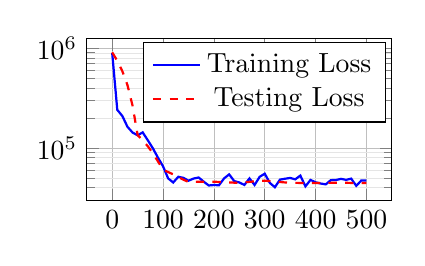
\begin{tikzpicture}
    \begin{axis}[
        width=0.45\textwidth,
        height=0.3\textwidth,
        % xlabel={Epochs},
        % ylabel={Loss},
        % Y logarithmic axis
        ymode=log,
        grid=both,
        grid style={line width=.1pt, draw=gray!20},
        major grid style={line width=.2pt,draw=gray!50},
    ]

    % Training Loss
    \addplot[color=blue, thick] table[row sep=\\] {
            Epoch Loss \\
            0 894546.0125 \\
            10 240647.390625 \\
            20 208289.765625 \\
            30 162688.459375 \\
            40 142362.18125 \\
            50 133538.4703125 \\
            60 142785.1875 \\
            70 119116.9234375 \\
            80 98903.753125 \\
            90 79687.421875 \\
            100 65185.97109375 \\
            110 49347.9375 \\
            120 44863.6984375 \\
            130 51181.3390625 \\
            140 49958.3921875 \\
            150 46749.040625 \\
            160 49113.27734375 \\
            170 50369.7625 \\
            180 45679.73125 \\
            190 41866.0859375 \\
            200 42301.59765625 \\
            210 42076.32109375 \\
            220 49279.109375 \\
            230 54109.38828125 \\
            240 46322.3109375 \\
            250 44875.58515625 \\
            260 42411.8765625 \\
            270 49259.47734375 \\
            280 42368.46875 \\
            290 51127.92109375 \\
            300 54962.2125 \\
            310 44441.3359375 \\
            320 40187.79453125 \\
            330 47953.93203125 \\
            340 48932.9765625 \\
            350 49824.9890625 \\
            360 48233.25390625 \\
            370 52632.85078125 \\
            380 41030.32734375 \\
            390 47593.34453125 \\
            400 45065.97109375 \\
            410 43793.12265625 \\
            420 42970.01953125 \\
            430 47376.1078125 \\
            440 47519.26484375 \\
            450 48781.07734375 \\
            460 47663.4484375 \\
            470 49045.4625 \\
            480 41527.11328125 \\
            490 47051.859375 \\
            500 47051.859375 \\
    };
    \addlegendentry{Training Loss}

    % Testing Loss
    \addplot[color=red, thick, dashed] table[row sep=\\] {
            Epoch Loss \\
            0 907952.7412288137 \\
            10 747379.7047881356 \\
            20 586806.6683474575 \\
            30 426233.6319067796 \\
            40 265660.59546610166 \\
            50 134148.47342955507 \\
            60 118880.00900953388 \\
            70 103611.5445895127 \\
            80 88343.08016949151 \\
            90 73074.61574947034 \\
            100 60242.12152542373 \\
            110 57153.50808527542 \\
            120 54064.89464512712 \\
            130 50976.28120497881 \\
            140 47887.667764830505 \\
            150 45428.732682733054 \\
            160 45488.51103283898 \\
            170 45548.28938294492 \\
            180 45608.06773305085 \\
            190 45667.84608315678 \\
            200 45666.05669226695 \\
            210 45417.99633739407 \\
            220 45169.93598252119 \\
            230 44921.8756276483 \\
            240 44673.81527277542 \\
            250 44570.649472987294 \\
            260 45047.061893538135 \\
            270 45523.47431408898 \\
            280 45999.88673463983 \\
            290 46476.299155190674 \\
            300 46765.07284427966 \\
            310 46303.29160752118 \\
            320 45841.51037076271 \\
            330 45379.72913400424 \\
            340 44917.94789724576 \\
            350 44537.04123411017 \\
            360 44479.6328654661 \\
            370 44422.22449682203 \\
            380 44364.81612817797 \\
            390 44307.4077595339 \\
            400 44275.25231726695 \\
            410 44344.10858050848 \\
            420 44412.96484375 \\
            430 44481.82110699153 \\
            440 44550.67737023305 \\
            450 44589.44007415255 \\
            460 44507.8285407839 \\
            470 44426.21700741526 \\
            480 44344.60547404661 \\
            490 44262.99394067797 \\
            500 44262.99394067797 \\
    };
    \addlegendentry{Testing Loss}
        
    \pgfplotsset{xtick={0,100,200,300,400,500}}

    \end{axis}
\end{tikzpicture}
\end{figure}



\begin{figure}[H]
    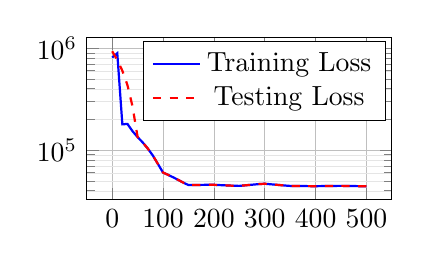
\begin{tikzpicture}
        \begin{axis}[
            width=0.45\textwidth,
            height=0.3\textwidth,
            % xlabel={Epochs},
            % ylabel={Loss},
            % Y logarithmic axis
            ymode=log,
            grid=both,
            grid style={line width=.1pt, draw=gray!20},
            major grid style={line width=.2pt,draw=gray!50},
        ]
    
        % Training Loss
    \addplot[color=blue, thick] table[row sep=\\] {
        Epoch Loss \\
        0 808947.237500 \\
        10 890469.778125 \\
        20 178986.278125 \\
        30 180629.865625 \\
        40 153239.050000 \\
        50 134148.473430 \\
        60 118880.009010 \\
        70 103611.544590 \\
        80 88343.080169 \\
        90 73074.615749 \\
        100 60242.121525 \\
        110 57153.508085 \\
        120 54064.894645 \\
        130 50976.281205 \\
        140 47887.667765 \\
        150 45428.732683 \\
        160 45488.511033 \\
        170 45548.289383 \\
        180 45608.067733 \\
        190 45667.846083 \\
        200 45666.056692 \\
        210 45417.996337 \\
        220 45169.935983 \\
        230 44921.875628 \\
        240 44673.815273 \\
        250 44570.649473 \\
        260 45047.061894 \\
        270 45523.474314 \\
        280 45999.886735 \\
        290 46476.299155 \\
        300 46765.072844 \\
        310 46303.291608 \\
        320 45841.510371 \\
        330 45379.729134 \\
        340 44917.947897 \\
        350 44537.041234 \\
        360 44479.632865 \\
        370 44422.224497 \\
        380 44364.816128 \\
        390 44307.407760 \\
        400 44275.252317 \\
        410 44344.108581 \\
        420 44412.964844 \\
        430 44481.821107 \\
        440 44550.677370 \\
        450 44589.440074 \\
        460 44507.828541 \\
        470 44426.217007 \\
        480 44344.605474 \\
        490 44262.993941 \\
        500 44262.993941 \\
};
\addlegendentry{Training Loss}

% Testing Loss
\addplot[color=red, thick, dashed] table[row sep=\\] {
        Epoch Loss \\
        0 931903.038363 \\
        10 765993.065985 \\
        20 600083.093607 \\
        30 434173.121229 \\
        40 268263.148851 \\
        50 134148.473430 \\
        60 118880.009010 \\
        70 103611.544590 \\
        80 88343.080169 \\
        90 73074.615749 \\
        100 60242.121525 \\
        110 57153.508085 \\
        120 54064.894645 \\
        130 50976.281205 \\
        140 47887.667765 \\
        150 45428.732683 \\
        160 45488.511033 \\
        170 45548.289383 \\
        180 45608.067733 \\
        190 45667.846083 \\
        200 45666.056692 \\
        210 45417.996337 \\
        220 45169.935983 \\
        230 44921.875628 \\
        240 44673.815273 \\
        250 44570.649473 \\
        260 45047.061894 \\
        270 45523.474314 \\
        280 45999.886735 \\
        290 46476.299155 \\
        300 46765.072844 \\
        310 46303.291608 \\
        320 45841.510371 \\
        330 45379.729134 \\
        340 44917.947897 \\
        350 44537.041234 \\
        360 44479.632865 \\
        370 44422.224497 \\
        380 44364.816128 \\
        390 44307.407760 \\
        400 44275.252317 \\
        410 44344.108581 \\
        420 44412.964844 \\
        430 44481.821107 \\
        440 44550.677370 \\
        450 44589.440074 \\
        460 44507.828541 \\
        470 44426.217007 \\
        480 44344.605474 \\
        490 44262.993941 \\
        500 44262.993941 \\
};
\addlegendentry{Testing Loss}
            
        \pgfplotsset{xtick={0,100,200,300,400,500}}
    
        \end{axis}
    \end{tikzpicture}
    \end{figure}
    
    
    
\begin{figure}[H]
    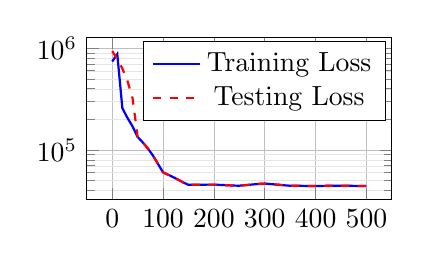
\begin{tikzpicture}
        \begin{axis}[
            width=0.45\textwidth,
            height=0.3\textwidth,
            % xlabel={Epochs},
            % ylabel={Loss},
            % Y logarithmic axis
            ymode=log,
            grid=both,
            grid style={line width=.1pt, draw=gray!20},
            major grid style={line width=.2pt,draw=gray!50},
        ]
    

    % Training Loss
    \addplot[color=blue, thick] table[row sep=\\] {
            Epoch Loss \\
            0 740167.537500 \\
            10 874002.806250 \\
            20 257119.903125 \\
            30 206597.973438 \\
            40 170604.325000 \\
            50 134148.473430 \\
            60 118880.009010 \\
            70 103611.544590 \\
            80 88343.080169 \\
            90 73074.615749 \\
            100 60242.121525 \\
            110 57153.508085 \\
            120 54064.894645 \\
            130 50976.281205 \\
            140 47887.667765 \\
            150 45428.732683 \\
            160 45488.511033 \\
            170 45548.289383 \\
            180 45608.067733 \\
            190 45667.846083 \\
            200 45666.056692 \\
            210 45417.996337 \\
            220 45169.935983 \\
            230 44921.875628 \\
            240 44673.815273 \\
            250 44570.649473 \\
            260 45047.061894 \\
            270 45523.474314 \\
            280 45999.886735 \\
            290 46476.299155 \\
            300 46765.072844 \\
            310 46303.291608 \\
            320 45841.510371 \\
            330 45379.729134 \\
            340 44917.947897 \\
            350 44537.041234 \\
            360 44479.632865 \\
            370 44422.224497 \\
            380 44364.816128 \\
            390 44307.407760 \\
            400 44275.252317 \\
            410 44344.108581 \\
            420 44412.964844 \\
            430 44481.821107 \\
            440 44550.677370 \\
            450 44589.440074 \\
            460 44507.828541 \\
            470 44426.217007 \\
            480 44344.605474 \\
            490 44262.993941 \\
            500 44262.993941 \\
    };
    \addlegendentry{Training Loss}

    % Testing Loss
    \addplot[color=red, thick, dashed] table[row sep=\\] {
            Epoch Loss \\
            0 935791.167055 \\
            10 782849.279873 \\
            20 629907.392691 \\
            30 476965.505508 \\
            40 324023.618326 \\
            50 134148.473430 \\
            60 118880.009010 \\
            70 103611.544590 \\
            80 88343.080169 \\
            90 73074.615749 \\
            100 60242.121525 \\
            110 57153.508085 \\
            120 54064.894645 \\
            130 50976.281205 \\
            140 47887.667765 \\
            150 45428.732683 \\
            160 45488.511033 \\
            170 45548.289383 \\
            180 45608.067733 \\
            190 45667.846083 \\
            200 45666.056692 \\
            210 45417.996337 \\
            220 45169.935983 \\
            230 44921.875628 \\
            240 44673.815273 \\
            250 44570.649473 \\
            260 45047.061894 \\
            270 45523.474314 \\
            280 45999.886735 \\
            290 46476.299155 \\
            300 46765.072844 \\
            310 46303.291608 \\
            320 45841.510371 \\
            330 45379.729134 \\
            340 44917.947897 \\
            350 44537.041234 \\
            360 44479.632865 \\
            370 44422.224497 \\
            380 44364.816128 \\
            390 44307.407760 \\
            400 44275.252317 \\
            410 44344.108581 \\
            420 44412.964844 \\
            430 44481.821107 \\
            440 44550.677370 \\
            450 44589.440074 \\
            460 44507.828541 \\
            470 44426.217007 \\
            480 44344.605474 \\
            490 44262.993941 \\
            500 44262.993941 \\
    };
    \addlegendentry{Testing Loss}
        \pgfplotsset{xtick={0,100,200,300,400,500}}
    
        \end{axis}
    \end{tikzpicture}
    \end{figure}
    
    
     

The x-axis has been truncated to 500 steps because the loss evolution of the
student models is not evolving much after that point. Hereafter we report the final
loss achieved by each model.

\begin{table}[H]
    \centering
    \begin{tabular}{|c|c|c|}
        \hline
        Model & Train Loss & Test Loss \\
        \hline
        $S_1$ & 47755 & 44895 \\
        $S_2$ & \textbf{42176} & 54148 \\
        $S_3$ & 47430 & \textbf{42891} \\
        \hline
    \end{tabular}
\end{table}
% \section{Exercise 2}

In this exercise, we will train a deep residual network on examples
generated by two specific functions. The first function is the 
6-dimensional multivariate complete Bell polynomial $B_6$, while
the second is the scrambled version of the first function $\tilde{B}_6$, as
described in the assignment.
\begin{align*}
    B_6(x_1, x_2, x_3, x_4, x_5, x_6) &= x_1^6 + 15x_2x_1^4 + 20x_3x_1^3 + 45x_2^2x_1^2 + 15x_2^3 \\
                                      &+ 60x_3x_2x_1 + 15x_4x_1^2 + 10x_3^2 + 15x_4x_2 \\
                                      &+ 6x_5x_1 + x_6 \\
\end{align*}


\subsection{Setup}

We begin by generating both the training and testing data for the two functions
by sampling from a uniform distribution and pass it through the functions.
\begin{align*}
    D_{train} &= \{(x_i, B_6(x_i))\}_{i=1}^{N}
    \\
    D_{test} &= \{(x_i, \tilde{B}_6(x_i))\}_{i=1}^{M}
    \\
    x_i &\sim \mathcal{U}(0, 1)^6
    \\
    N &= 10^5 \\
    M &= 6 \cdot 10^4
\end{align*}


\subsection{Training}

We use a nine-layers fully connected residual neural network and we train
it for 30 epochs with a batch size of 20. As usual, we use the Adam optimizer
and the mean squared error loss function. The learning rate is set to $10^{-3}$.
Hereafter we report the loss evolution plots for the training and testing data.

\begin{figure}[H]
    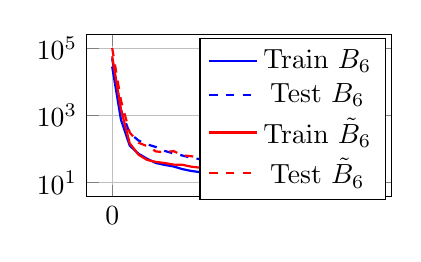
\begin{tikzpicture}
        \begin{axis}[
            width=0.45\textwidth,
            height=0.3\textwidth,
            % xlabel={Epochs},
            % ylabel={Loss},
            % Y logarithmic axis
            ymode=log,
            grid=both,
            grid style={line width=.1pt, draw=gray!20},
            major grid style={line width=.2pt,draw=gray!50},
        ]

    
        % Training Loss
    \addplot[color=blue, thick] table[row sep=\\] {
        Epoch Loss \\
        0 28222.798557 \\
        1 750.183850 \\
        2 127.187630 \\
        3 72.989227 \\
        4 51.318768 \\
        5 38.632868 \\
        6 33.888173 \\
        7 30.501737 \\
        8 25.455874 \\
        9 22.495250 \\
        10 20.716813 \\
        11 20.439270 \\
        12 19.947380 \\
        13 19.666327 \\
        14 18.084223 \\
        15 15.874462 \\
        16 14.237747 \\
        17 14.069838 \\
        18 13.702041 \\
        19 12.426478 \\
        20 12.481813 \\
        21 12.984934 \\
        22 11.525879 \\
        23 9.839362 \\
        24 10.819127 \\
        25 12.222121 \\
        26 12.444951 \\
        27 12.763526 \\
        28 11.970101 \\
        29 11.970101 \\
};
\addlegendentry{Train $B_6$}

% Testing Loss
\addplot[color=blue, thick, dashed] table[row sep=\\] {
        Epoch Loss \\
        0 49322.988180 \\
        1 1435.766413 \\
        2 297.219495 \\
        3 180.150779 \\
        4 138.309639 \\
        5 115.138365 \\
        6 88.188905 \\
        7 74.261032 \\
        8 64.503982 \\
        9 55.510019 \\
        10 50.215417 \\
        11 51.448758 \\
        12 49.441075 \\
        13 67.158930 \\
        14 63.096009 \\
        15 36.855787 \\
        16 35.294025 \\
        17 36.094313 \\
        18 34.141850 \\
        19 29.649502 \\
        20 33.677476 \\
        21 34.482947 \\
        22 29.191524 \\
        23 26.037694 \\
        24 27.380395 \\
        25 26.073013 \\
        26 23.682013 \\
        27 21.019013 \\
        28 18.978013 \\
        29 15.874462 \\
};
\addlegendentry{Test $B_6$}

% Training Loss
\addplot[color=red, thick] table[row sep=\\] {
        Epoch Loss \\
        0 57108.709374 \\
        1 1511.709526 \\
        2 149.337356 \\
        3 68.204837 \\
        4 47.521360 \\
        5 41.628717 \\
        6 38.568051 \\
        7 34.665786 \\
        8 34.209594 \\
        9 30.142201 \\
        10 28.078693 \\
        11 26.964283 \\
        12 27.384413 \\
        13 23.730984 \\
        14 24.259848 \\
        15 23.298907 \\
        16 22.388610 \\
        17 22.762765 \\
        18 21.351404 \\
        19 20.827035 \\
        20 20.278060 \\
        21 20.803791 \\
        22 17.897703 \\
        23 22.126576 \\
        24 19.848122 \\
        25 18.528484 \\
        26 21.716314 \\
        27 20.972649 \\
        28 25.436561 \\
        29 21.018406 \\
};
\addlegendentry{Train $\tilde{B}_6$}

% Testing Loss
\addplot[color=red, thick, dashed] table[row sep=\\] {
    Epoch Loss \\
    0 100483.626753 \\
    1 2800.730182 \\
    2 311.694159 \\
    3 155.007909 \\
    4 122.048066 \\
    5 85.218807 \\
    6 80.762722 \\
    7 87.476556 \\
    8 65.439050 \\
    9 61.477907 \\
    10 56.790878 \\
    11 48.564881 \\
    12 42.752009 \\
    13 49.242996 \\
    14 39.044080 \\
    15 44.229642 \\
    16 42.250782 \\
    17 40.528426 \\
    18 42.540765 \\
    19 38.004709 \\
    20 39.475441 \\
    21 38.155473 \\
    22 30.061123 \\
    23 48.899072 \\
    24 43.116610 \\
    25 35.323654 \\
    26 35.537259 \\
    27 47.725050 \\
    28 42.262133 \\
    29 39.588323 \\
};
\addlegendentry{Test $\tilde{B}_6$}
    
        \end{axis}
    \end{tikzpicture}
    \end{figure}
    
    
    
\begin{table}[H]
    \centering
    \begin{tabular}{c|cc}
        \toprule
        \textbf{Function} & Train Loss & Test Loss \\
        \midrule
        $B_6$ & \textbf{11.97} & \textbf{15.87} \\
        $\tilde{B}_6$ & 21.02 & 39.59 \\
        \bottomrule
    \end{tabular}
\end{table}

As we can see from the plots and the table, the network is able to learn
more easily the first function $B_6$ than the second $\tilde{B}_6$.
This provides empirical evidence in favor of the hypothesis that the
neural networks better approximate hierarchical compositional
functions. \\

If we then fix five of the six input variables, make the free variable
vary in the range $[0, 2]$ and plot the loss function, we obtain the following
plot.
\begin{figure}[H]
    \begin{tikzpicture}
        \begin{axis}[
            width=0.45\textwidth,
            height=0.3\textwidth,
            ymode=log,
            % legend north west
            legend pos=north west,
            xmin=0,
            xmax=2,
            grid=both,
            grid style={line width=.1pt, draw=gray!20},
            major grid style={line width=.2pt,draw=gray!50},
        ]

        % Training Loss
        \addplot[color=blue, thick] table[row sep=\\] {
            0 5.863006 \\
            0.1 0.076559 \\
            0.2 1.126767 \\
            0.3 1.781454 \\
            0.4 0.929033 \\
            0.5 1.718634 \\
            0.6 7.983808 \\
            0.7 6.881893 \\
            0.8 1.146498 \\
            0.9 4.260346 \\
            1.0 12.809544 \\
            1.1 11.848450 \\
            1.2 2.623605 \\
            1.3 2.404091 \\
            1.4 3.087926 \\
            1.5 1.298338 \\
            1.6 0.849399 \\
            1.7 1.620012 \\
            1.8 8.973556 \\
            1.9 1.197073 \\
            2.0 2.197073 \\
        };
        \addlegendentry{$B_6$}

        % Training Loss
        \addplot[color=red, thick] table[row sep=\\] {
            0 2.956828e+02 \\
            0.1 2.977129e+03 \\
            0.2 1.459246e+04 \\
            0.3 4.114617e+03 \\
            0.4 2.189786e+04 \\
            0.5 1.180784e+04 \\
            0.6 6.035422e+02 \\
            0.7 3.895891e+03 \\
            0.8 1.219255e+05 \\
            0.9 1.017331e+04 \\
            1.0 2.994255e+04 \\
            1.1 4.837233e+04 \\
            1.2 4.672473e+05 \\
            1.3 3.557021e+05 \\
            1.4 8.204140e+05 \\
            1.5 4.601622e+05 \\
            1.6 7.368604e+04 \\
            1.7 2.065889e+06 \\
            1.8 9.732446e+05 \\
            1.9 4.026183e+05 \\
            2.0 4.326183e+05 \\
        };
        \addlegendentry{$\tilde{B}_6$}

        \end{axis}
    \end{tikzpicture}
\end{figure}


Which shows that the network is able to generalize well to perturbations
of the input data when considering the function $B_6$, but not when
considering the function $\tilde{B}_6$.

\section{Conclusions}
In this report we have seen how Kernel PCA can be used to reduce the
dimensionality of the data and how it can outperform PCA when the data
lies in a non-linear manifold.
We have also seen how unsupervised learning can be used to retrieve
labels from the data and how these labels can be used to train classifiers.
Finally, we have seen how the performance of the classifiers can improve
when trained on the original labels.